\documentclass[12pt]{article}
\usepackage{Diploma}


\begin{document}

{
\renewcommand{\baselinestretch}{1}
\thispagestyle{empty}
\begin{center}
    
        Федеральное государственное автономное образовательное учреждение\\
        высшего образования\\
        "Московский физико-технический институт\\
        {\rm(национальный исследовательский университет)}"\\
        Физтех-школа прикладной математики и информатики\\
        Кафедра интеллектуальных систем\\[35mm]
    \rm\large
        Северилов Павел Андреевич\\[10mm]
    \bf\Large
        Выбор оптимальной модели в задаче моделирования\\
        динамики физической системы\\[10mm]
    \rm\normalsize
        03.04.01 --- Прикладные математика и физика\\[10mm]
    \sc
        Магистерская диссертация\\[30mm]
\end{center}
\hfill\parbox{80mm}{
    \begin{flushleft}
    \bf
        Научный руководитель:\\
    \rm
        д. ф.-м. н.\\
        Стрижов Вадим Викторович\\[3cm]
    \end{flushleft}
}
\begin{center}
    Москва\\
    2022 г.
\end{center}
}

\newpage
\tableofcontents

\newpage
\begin{abstract}
	В работе решается задача выбора оптимальной модели предсказания динамики физической системы. Под динамикой системы понимается изменение во времени параметров системы. Нейронные сети не имеют априорных знаний о моделируемой системе, что не позволяет получить оптимальные параметры, учитывающие физические законы. Лагранжева нейронная сеть учитывает закон сохранения энергии при моделировании динамики. В данной работе предлагается Нётеровская агранжева нейронная сеть, учитывающая законы сохранения импульса и момента импульса в дополнение к закону сохранения энергии. Показано, что для данной задачи Нётеровская Лагранжева нейронная сеть является оптимальной среди полносвязной модели нейронной сети, нейронной сети с долговременной кратковременной памятью и Лагранжевой нейронной сетью. Сравнение моделирования проводилось на искусственно сгенерированных данных для системы двойного маятника, которая является простейшей хаотической системой. Результаты экспериментов подтверждают гипотезу, что внесение априорного знания о физике системы повышает качество модели.

\end{abstract}

\newpage
%%%%%%%%%%%%%%%%%%%%%%%%%%%%%%%%%%%%%%%%%%%%%%%%%%%%%%%%%%%%%%%%%%%%%%%%%%
\section{Введение}
%%%%%%%%%%%%%%%%%%%%%%%%%%%%%%%%%%%%%%%%%%%%%%%%%%%%%%%%%%%%%%%%%%%%%%%%%%


Моделирование динамики физической системы является одной из основных задач механики \cite{goldstein:mechanics, arnold_mechanics}. Под динамикой системы понимается изменение во времени параметров этой системы.

В классической механике, чтобы получить динамику системы, необходимо расписать все силы системы, уравнения сохранения импульса и энергии и численно решить полученные дифференциальные уравнения. Однако на практике моделирование динамики данным способом представляется затруднительным. Например, для хаотических систем: системы двойного маятника, системы трех тел.

Существующие модели решения обыкновенных дифференциальных уравнений с помощью нейронных сетей не имеют априорных знаний о моделируемой системе \cite{712178, NEURIPS2018_69386f6b}. Это не позволяет получить оптимальные параметры модели, которые учитывают физические законы \cite{hnnpaper, Cranmer2020LagrangianNN, delan}.

Альтернативным классической механике подходом является лагранжева динамика \cite{goldstein:mechanics}, которая переформулирует проблему в терминах набора обобщенных координат, которые полностью описывают возможные движения частицы. Чтобы использовать лагранжеву динамику, необходимо построить лагранжиан $L$, который определяется как разница между кинетической энергией ($T$) и потенциальной энергией ($V$) системы:
$$L = T - V $$

Интеграл $L$ по времени называется \textit{действием}. Истинная траектория системы минимизирует этот интеграл (\textit{принцип наименьшего действия}). Отсюда следует, что действие не может меняться при малых вариациях пути, что эквивалентно уравнению Эйлера-Лагранжа
$$
\frac{\partial L}{\partial x}-\frac{d}{d t} \frac{\partial L}{\partial \dot{x}}=0
$$

Лагранжевы нейронные сети (LNN) \cite{Cranmer2020LagrangianNN, delan} основаны на лагранжевой динамике. Модель аппроксимирует лагранжиан системы, из которого с помощью уравнения Эйлера-Лагранжа получается динамика системы. Таким образом, LNN имет априорные знания о моделируемой системе в виде её лагранжиана. 

В модели LNN лагранжиан независим от времени, т.е. учитывается закон сохранения энергии. Но не учитываются другие законы сохранения, как закон сохранения импульса и момента импульса.

Теорема Нетер \cite{doi:10.1080/00411457108231446} говорит о том, что любая непрерывная симметрия лагранжиана $L$ связана с сохраняющейся величиной системы.  Например, если $L$ не меняется при трансляции (т. е. обладает трансляционной симметрией), то сохраняется импульс. Если $L$ не меняется при поворотах, то сохраняется момент импульса. Таким образом, в терминах теоремы Нётер LNN имеет временную трансляционную симметрию, но не имеет трансляционной и вращательной симметрий.

В данной работе предлагается Нётеровская нейронная сеть, которая является модификацией Лагранжевой нейронной сети, в которой учитываются трансляционные и вращательные симметрии. Модель получает на вход разницу координат вместо самих координат и аппроксимирует потенциальную энергию системы. Лагранжиан системы в таком случае будет разностью известной кинетической энергии и аппроксимированной потенциальной энергией. Показано, что при такой постановке, лагранжиан системы будет инвариантен относительно трансляции и поворотов в пространстве.

Для вычислительного эксперимента была взята простейшая хаотическая система двойного маятника \cite{arnold_mechanics}. В данной системе сохраняется энергия, импульс и момент импульса \cite{class_mechanics}. Для моделирования динамики системы были взяты полносвязная нейронная сеть\cite{SCHMIDHUBER201585}, нейронная сеть с долгой краткосрочной памятью (LSTM) \cite{lstm}, LNN \cite{Cranmer2020LagrangianNN} и Нётеровская LNN. Результаты моделирования сравнивались с траекториями маятника, полученными аналитическим решением с помощью метода Рунге-Кутты 4-ого порядка \cite{runge_kutta}. Показано, что качество моделирования динамики системы повышается при добавлении априорного знания о физике системы.


%%%%%%%%%%%%%%%%%%%%%%%%%%%%%%%%%%%%%%%%%%%%%%%%%%%%%%%%%%%%%%%%%%%%%%%%%%
\section{Постановка задачи регрессии динамики физической системы}
%%%%%%%%%%%%%%%%%%%%%%%%%%%%%%%%%%%%%%%%%%%%%%%%%%%%%%%%%%%%%%%%%%%%%%%%%%
Задачу моделирования динамики системы можно свести к задаче регрессии.
Пусть дана выборка из $m$ траекторий 
$$\left\{\mathbf{x}_i, \mathbf{y}_i\right\}_{i=1}^m,$$ где $\mathbf{x}_i = (\mathbf{q}_i, \mathbf{\dot{q}}_i)$~--  координаты траектории движения двойного маятника, $\mathbf{{y}}_i = \mathbf{\dot{x}}_i = (\mathbf{\dot{q}}_i, \mathbf{\ddot{q}}_i)$ -- динамика движения системы двойного маятника, $\mathbf{q}_i \in \mathbb{R}^{r \times n}$, где $r$ -- количество координат, $n$ -- длина траектории.

Регрессионная модель выбирается из класса нейронных сетей
$$\{\mathbf{f}_k\colon(\mathbf{w}, \mathbf{X})\to  \hat{\mathbf{y}} \mid k \in \mathcal{K}\},$$ где $\mathbf{w} \in \mathbb{W}$~-- параметры модели, $\hat{\mathbf{y}} = \mathbf{f} (\mathbf{X},\mathbf{w}) \in \mathbb{R}^{2\times r \times n}, \mathbf{X} = \bigcup_{i=1}^m \mathbf{x}_i$.

В качестве функция ошибки взята квадратичная ошибка: 
$$\mathcal{L}(\mathbf{y}, \mathbf{X}, \mathbf{w}) =\left\lVert \hat{\mathbf{y}} - \mathbf{y} \right\rVert^{2}_2.$$

Таким образом, задача моделирования динамики системы представлена в виде задачи минимизации квадратичной ошибки: 
$$\textbf{w}^* = \underset{\mathbf{w}\in\mathbb{W}}{\text{argmin}}\bigl(\mathcal{L}(\textbf{w})\bigr).$$


%%%%%%%%%%%%%%%%%%%%%%%%%%%%%%%%%%%%%%%%%%%%%%%%%%%%%%%%%%%%%%%%%%%%%%%%%%
\section{Лагранжевы нейронные сети}
%%%%%%%%%%%%%%%%%%%%%%%%%%%%%%%%%%%%%%%%%%%%%%%%%%%%%%%%%%%%%%%%%%%%%%%%%%
\subsection{Лагранжева динамика}		

Лагранжев формализм \cite{Cranmer2020LagrangianNN, goldstein:mechanics, class_mechanics, arnold_mechanics} моделирует физическую систему с координатами $x_t = (q, \dot{q})$, которая начинается в состоянии $x_0$ и заканчивается в другом состоянии $x_1$. Определяется функционал, который называется действием
$$S=\int_{t_{0}}^{t_{1}} L d t,$$
 где $L$ -- лагранжиан системы. Действие определяет путь, по которому координаты $x_t$ пройдут из $x_0$ в $x_1$ в промежуток времени от $t_0$ до $t_1$. Путь минимизирует действие $S$, т.е. $\delta S = 0$. Это приводит к уравнению Эйлера-Лагранжа, определяющему динамику системы
$$\frac{d}{d t} \frac{\partial L}{\partial \dot{\mathbf{q}}}=\frac{\partial L}{\partial \mathbf{q}}$$

Ускорение каждой компоненты системы $ \ddot{\mathbf{q}}$ может быть напрямую получено из данного уравнения:

$$\begin{aligned} 
\frac{\partial}{\partial \dot{\mathbf{q}}} \frac{d L}{d t} 
&=\frac{\partial L}{\partial \mathbf{q}} \\ \frac{\partial}{\partial \dot{\mathbf{q}}}\left(\frac{\partial L}{\partial \mathbf{q}} \frac{d q}{d t}+\frac{\partial L}{\partial \dot{\mathbf{q}}} \frac{d \dot{\mathbf{q}}}{d t}\right) 
&=\frac{\partial L}{\partial \mathbf{q}} \\ \frac{\partial}{\partial \dot{\mathbf{q}}}\left(\frac{\partial L}{\partial \mathbf{q}} \dot{\mathbf{q}}+\frac{\partial L}{\partial \dot{\mathbf{q}}} \ddot{\mathbf{q}}\right) 
&=\frac{\partial L}{\partial \mathbf{q}} \\ \frac{\partial}{\partial \dot{\mathbf{q}}} \frac{\partial L}{\partial \mathbf{q}} \dot{\mathbf{q}}+\frac{\partial}{\partial \dot{\mathbf{q}}} \frac{\partial L}{\partial \dot{\mathbf{q}}} \ddot{\mathbf{q}} 
&=\frac{\partial L}{\partial \mathbf{q}} \\ \frac{\partial}{\partial \dot{\mathbf{q}}} \frac{\partial L}{\partial \dot{\mathbf{q}}} \ddot{\mathbf{q}} 
&=\frac{\partial L}{\partial \mathbf{q}}-\frac{\partial}{\partial \dot{\mathbf{q}}} \frac{\partial L}{\partial \mathbf{q}} \dot{\mathbf{q}} \\ \ddot{\mathbf{q}} 
&=\left(\frac{\partial}{\partial \dot{\mathbf{q}}} \frac{\partial L}{\partial \dot{\mathbf{q}}}\right)^{-1}\left[\frac{\partial L}{\partial \mathbf{q}}-\frac{\partial}{\partial \dot{\mathbf{q}}} \frac{\partial L}{\partial \mathbf{q}} \dot{\mathbf{q}}\right] \\ \ddot{\mathbf{q}} 
&=\left(\nabla_{\dot{\mathbf{q}} \dot{\mathbf{q}}} L\right)^{-1}\left[\nabla_{q} L-\left(\nabla_{\dot{\mathbf{q}}\mathbf{q}} L\right) \dot{\mathbf{q}}\right],
\end{aligned}$$

где гессиан $\left(\nabla_{\dot{\mathbf{q}\mathbf{q}}} L\right)_{i j}=\frac{\partial^{2} L}{\partial q_{j} \partial \dot{q}_{i}}$.

Таким образом, алгоритм моделирования динамики системы в лагранжевой динамике:
\begin{enumerate}
	\item Найти аналитические выражения для кинетической $(T)$ и потенциальной энергии $(V)$
	\item Получить лагранжиан $\mathcal{L} = T - V $
	\item Применить ограничение Эйлера-Лагранжа $\frac{d}{d t} \frac{\partial L}{\partial \mathbf{\dot{q}}} =\frac{\partial L}{\partial \mathbf{q}} $
	\item Решить получившуюся систему дифференциальных уравнений
\end{enumerate}


\subsection{Лагранжевы нейронные сети}

В работе \cite{Cranmer2020LagrangianNN} предложено в нейронную сеть $$f: \mathbf{X} = (\mathbf{q}, \mathbf{\dot{q}}) \rightarrow \mathbf{Y}$$
 добавить априорные знания о физике системы, учитывая лагранжиан системы:
$$f: \mathbf{X} = (\mathbf{q}, \mathbf{\dot{q}}) \rightarrow \mathbf{L};$$

Т.е. ключевой идеей является параметризовать нейронной сетью лагранжиан $L$, получить выражение ограничения Эйлера-Лагранжа и обратно распространить ошибку через полученные ограничения
$$\ddot{\mathbf{q}} =\left(\nabla_{\dot{\mathbf{q}} \dot{\mathbf{q}}} L\right)^{-1}\left[\nabla_{q} L-\left(\nabla_{\dot{\mathbf{q}}\mathbf{q}} L\right) \dot{\mathbf{q}}\right],$$ 

На рисунке \ref{fig: base_vs_lnn} представлены схемы работы базового решения нейронными сетями и LNN для задачи моделирования динамики системы.На основе базового решения основаны работы \cite{NEURIPS2018_69386f6b, 712178}.

\begin{figure}[H]
	\centering
	\begin{subfigure}[b]{0.49\textwidth}
		\centering
		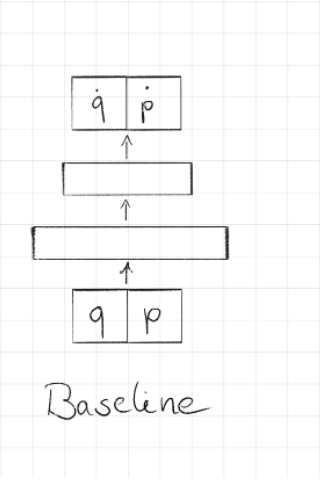
\includegraphics[width=0.55\textwidth]{baseline_nn_scheme.png}
		\caption{Базовое решение нейронными сетями}
		\label{fig:y equals x}
	\end{subfigure}
	\hfill
	\begin{subfigure}[b]{0.49\textwidth}
		\centering
		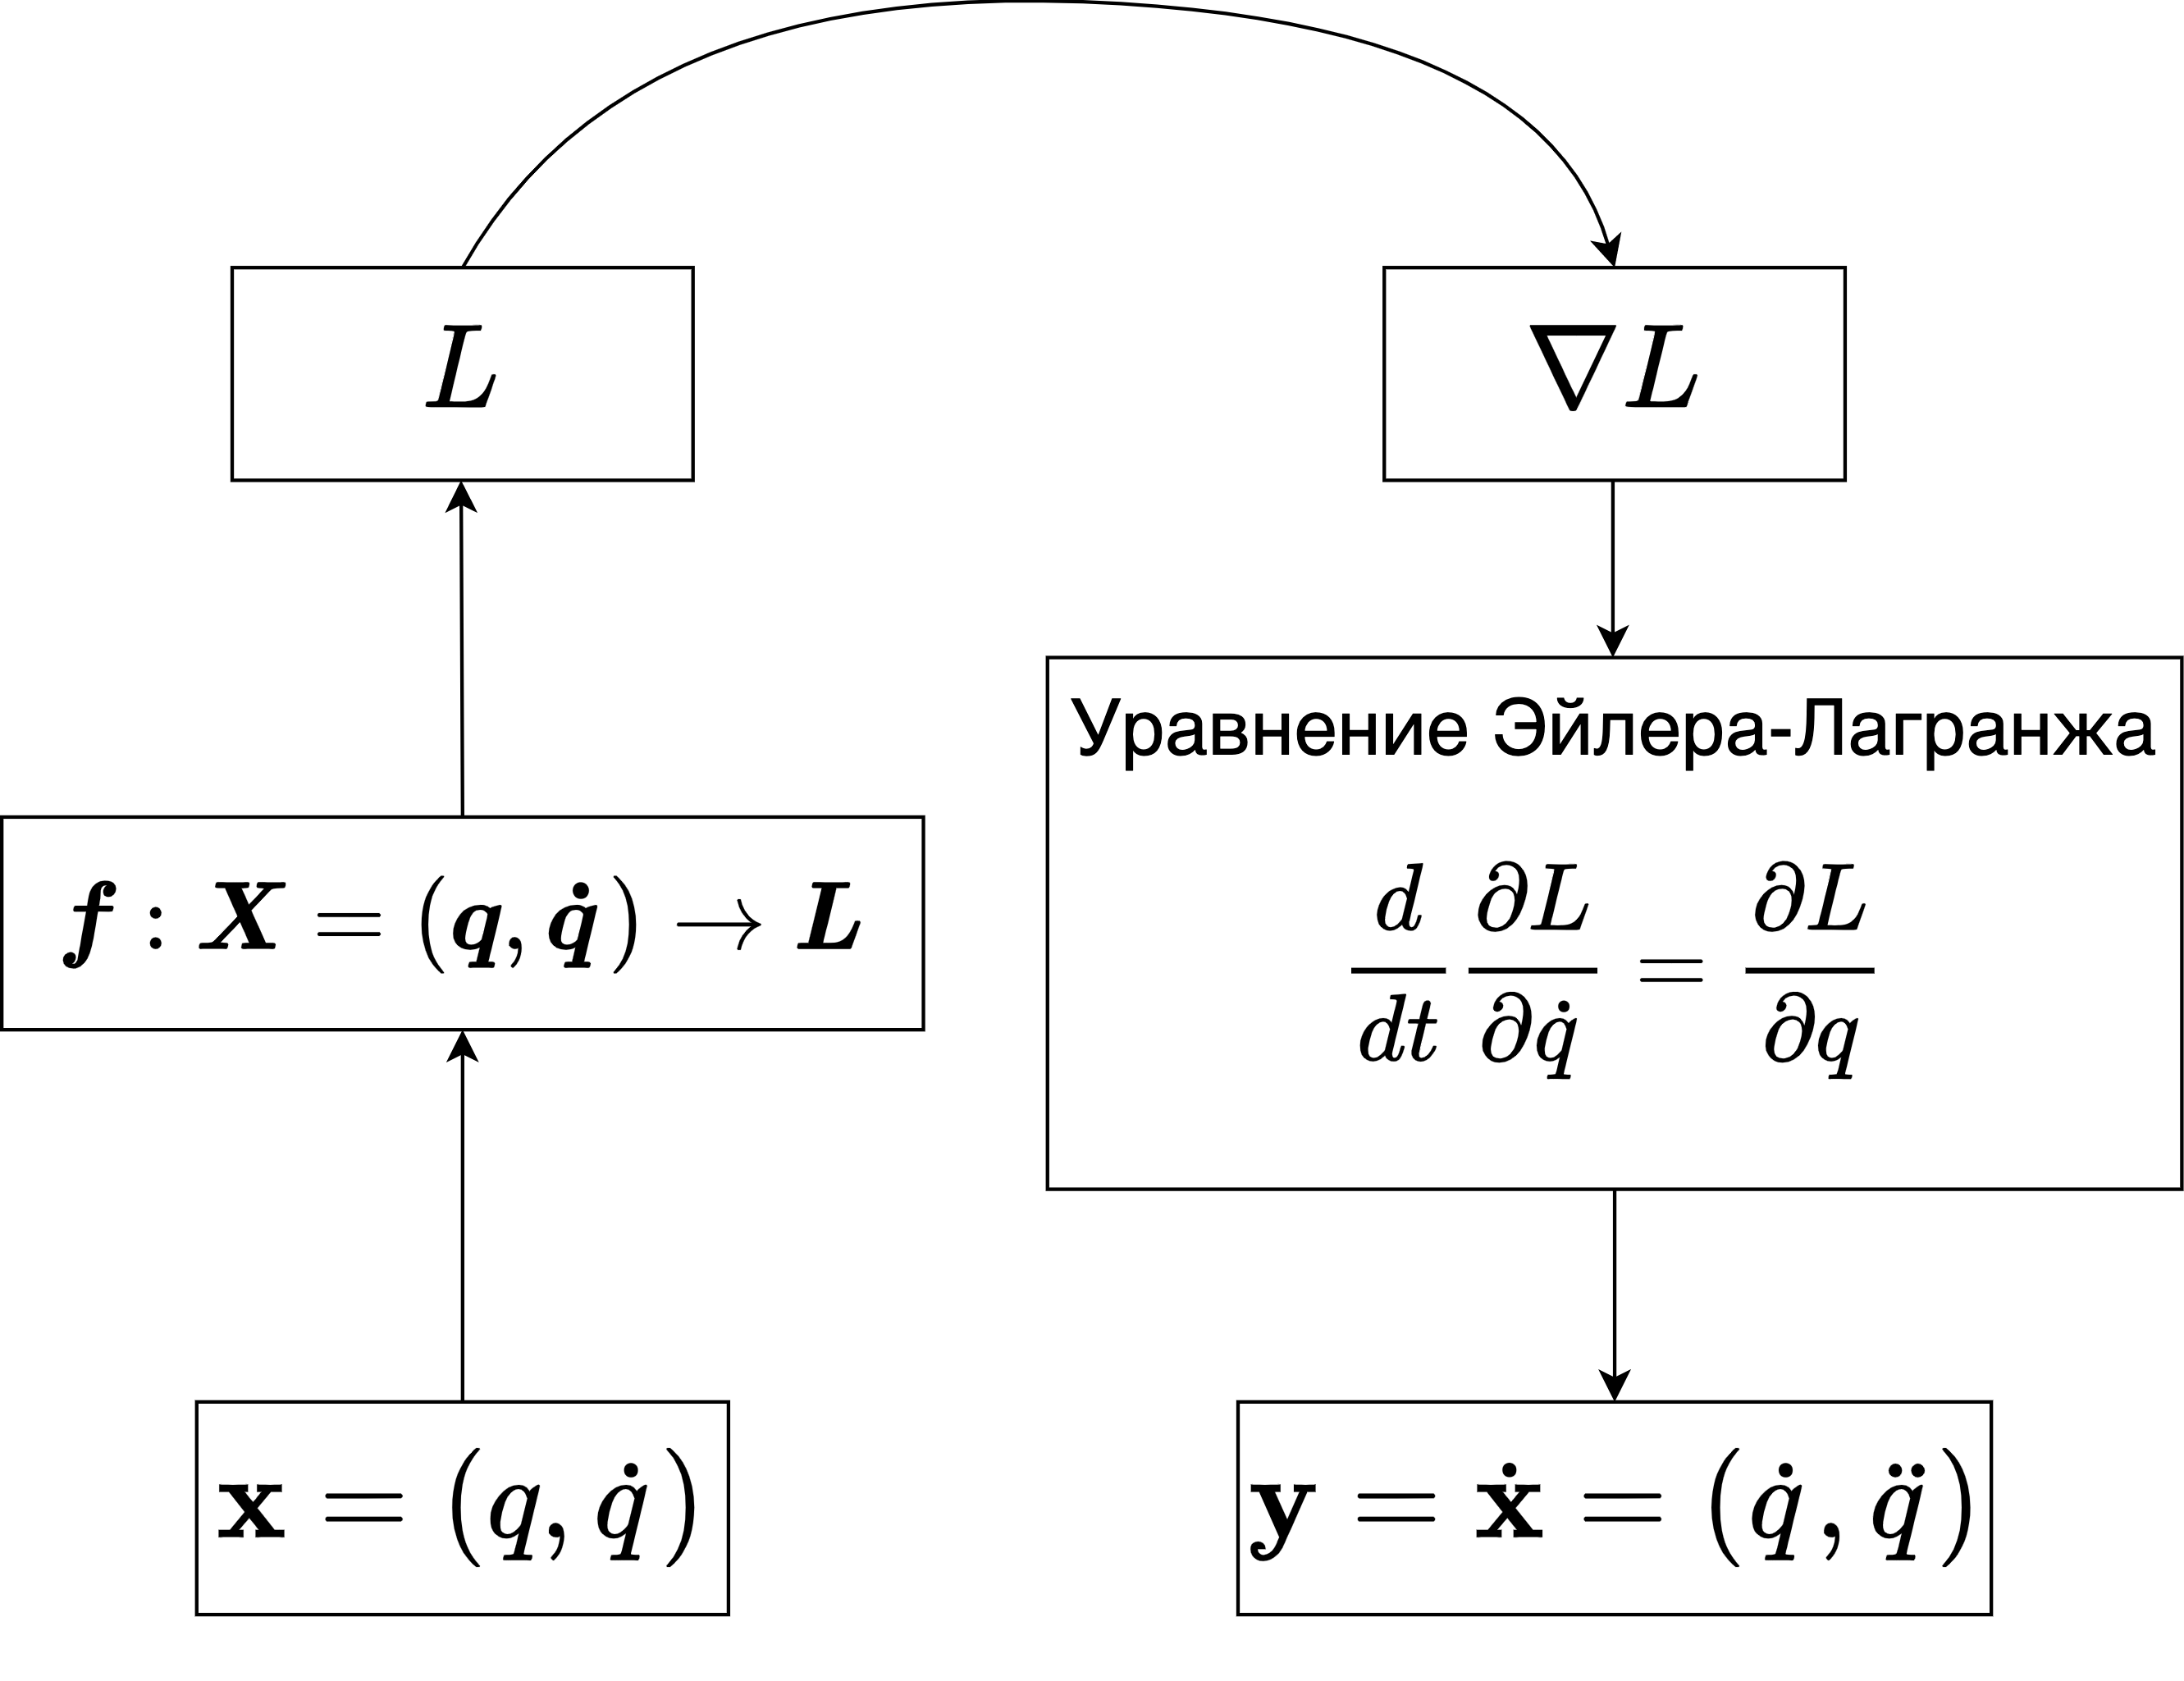
\includegraphics[width=\textwidth]{lnn_scheme.png}
		\caption{Решение LNN}
		\label{fig:three sin x}
	\end{subfigure}
\caption{Схемы работы базового решения нейронными сетями (a) и LNN (b) для задачи моделирования динамики физической системы}
\label{fig: base_vs_lnn}
\end{figure}

В качестве нейронной сети $f: \mathbf{X} = (\mathbf{q}, \mathbf{\dot{q}}) \rightarrow \mathbf{L}$ берется полносвязная сеть с 3-мя слоями. Таким образом, для заданных координат  $(\mathbf{q}, \mathbf{\dot{q}})$ имеем модель с априорными знанями о законе сохранения энергии, которой можем получить динамику параметров $(\mathbf{\dot{q}}, \mathbf{\ddot{q}})$.

%%%%%%%%%%%%%%%%%%%%%%%%%%%%%%%%%%%%%%%%%%%%%%%%%%%%%%%%%%%%%%%%%%%%%%%%%%
\section{Нётеровская Лагранжева нейронная сеть}
%%%%%%%%%%%%%%%%%%%%%%%%%%%%%%%%%%%%%%%%%%%%%%%%%%%%%%%%%%%%%%%%%%%%%%%%%%

Лагранжева нейронная сеть не обладает трансляционной и вращательной симметриями в пространстве. Предлагается \textit{Нётеровская Лагранжева нейронная сеть (LNN)}, которая получает на вход разницу между координатами элементов системы
$$\Delta q_{ij} =\sqrt{\left(\vec{q}_{i}-\vec{q}_{j}\right) \cdot\left(\vec{q}_{i}-\vec{q}_{j}\right)}  $$
и аппроксимирует потенциальную энергию системы $\boldsymbol{V}(\Delta \boldsymbol{q})$:
$$f: \boldsymbol{X} = (\boldsymbol{\Delta q})\rightarrow \boldsymbol{V},$$


В общем случае, Лагранжиан системы, получаемый Нётеровской LNN представим в виде
$$ L(\mathbf{\Delta q}, \mathbf{\dot{q}}) = T(\mathbf{\Delta q}, \mathbf{\dot{q}}) - V(\mathbf{\Delta q})$$

В общем виде, кинетическая энергия системы может быть получена аналитически для большинства систем:
$$T(\mathbf{\Delta q}, \mathbf{\dot{q}}) =\sum_{i=1}^{r} \frac{1}{2} m_{i} \dot{\vec{q}}_{i}^{2}$$

На рисунке \ref{fig: lnn_vs_noetherlnn} представлены схемы работы LNN и Нётеровской LNN для задачи моделирования динамики системы. Красным цветом наглядно показано отличие LNN от Нётеровской модификации: вместо лагранжиана параметризуется потенциальная энергия.  

\begin{figure}[H]
	\begin{subfigure}[b]{0.49\textwidth}
		\centering
		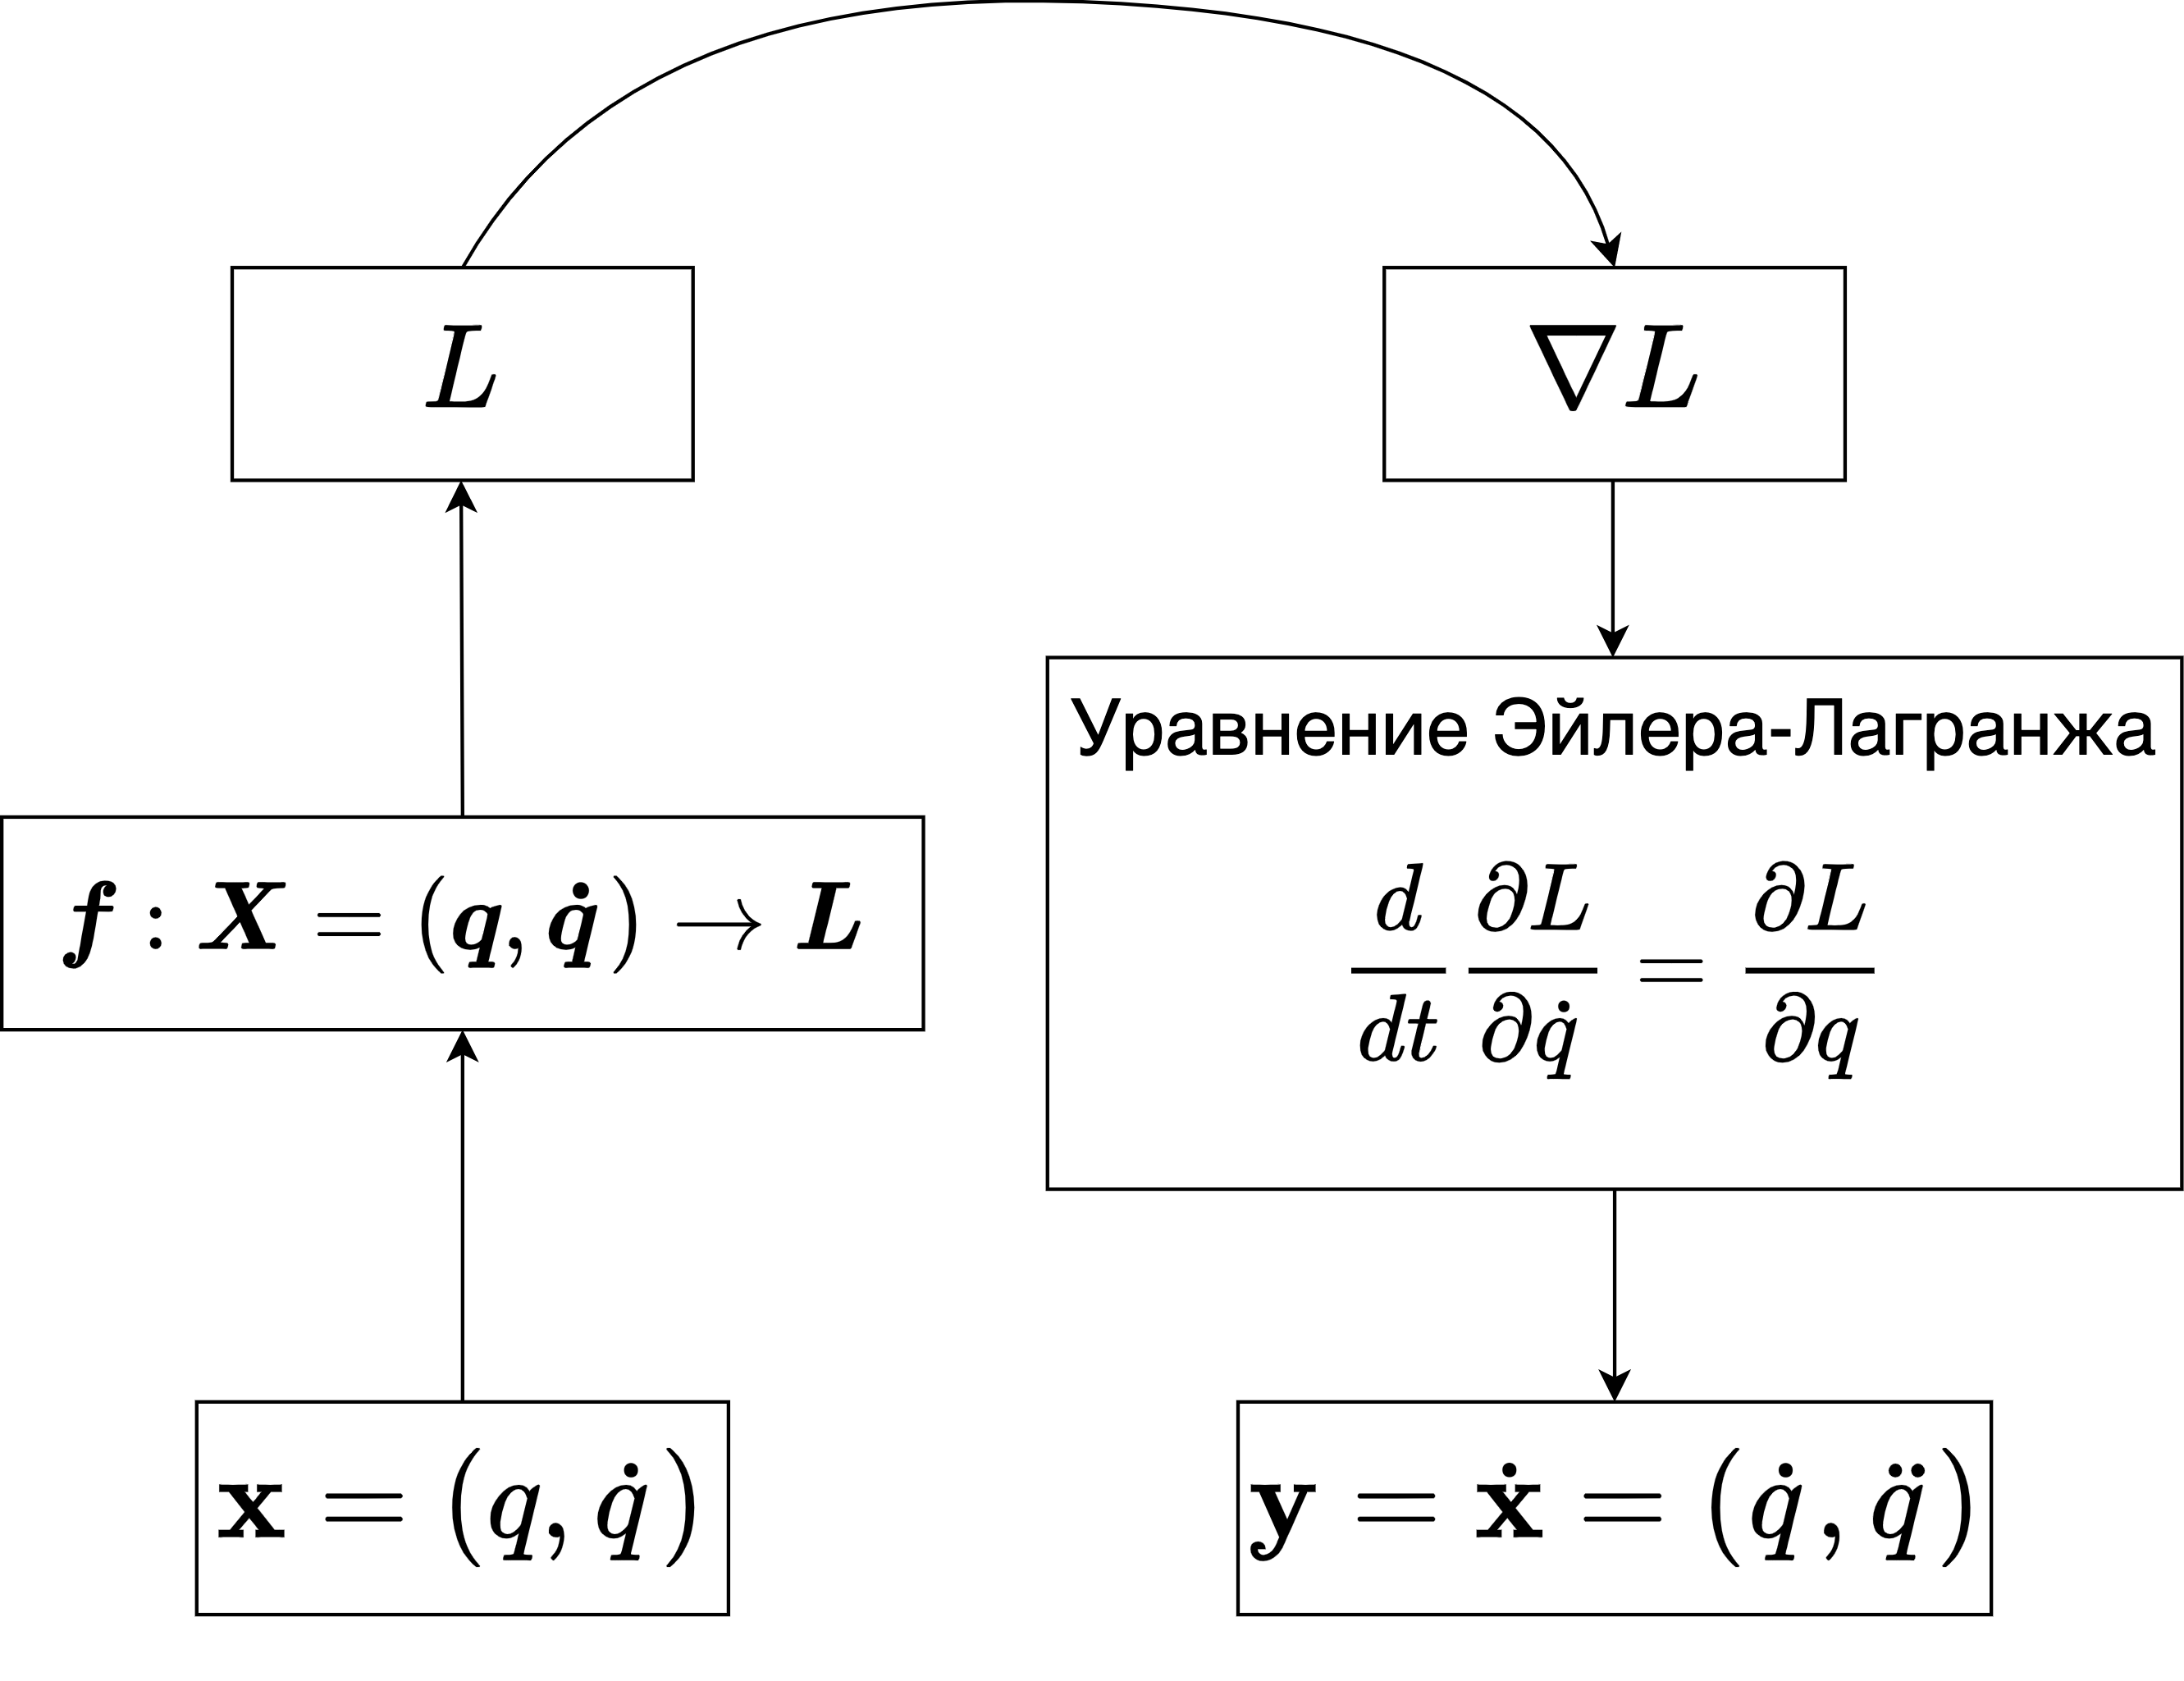
\includegraphics[width=0.99\textwidth]{lnn_scheme.png}
		\caption{Схема работы LNN}
		%\label{fig:y equals x}
	\end{subfigure}
	\hfill
	\begin{subfigure}[b]{0.49\textwidth}
		\centering
		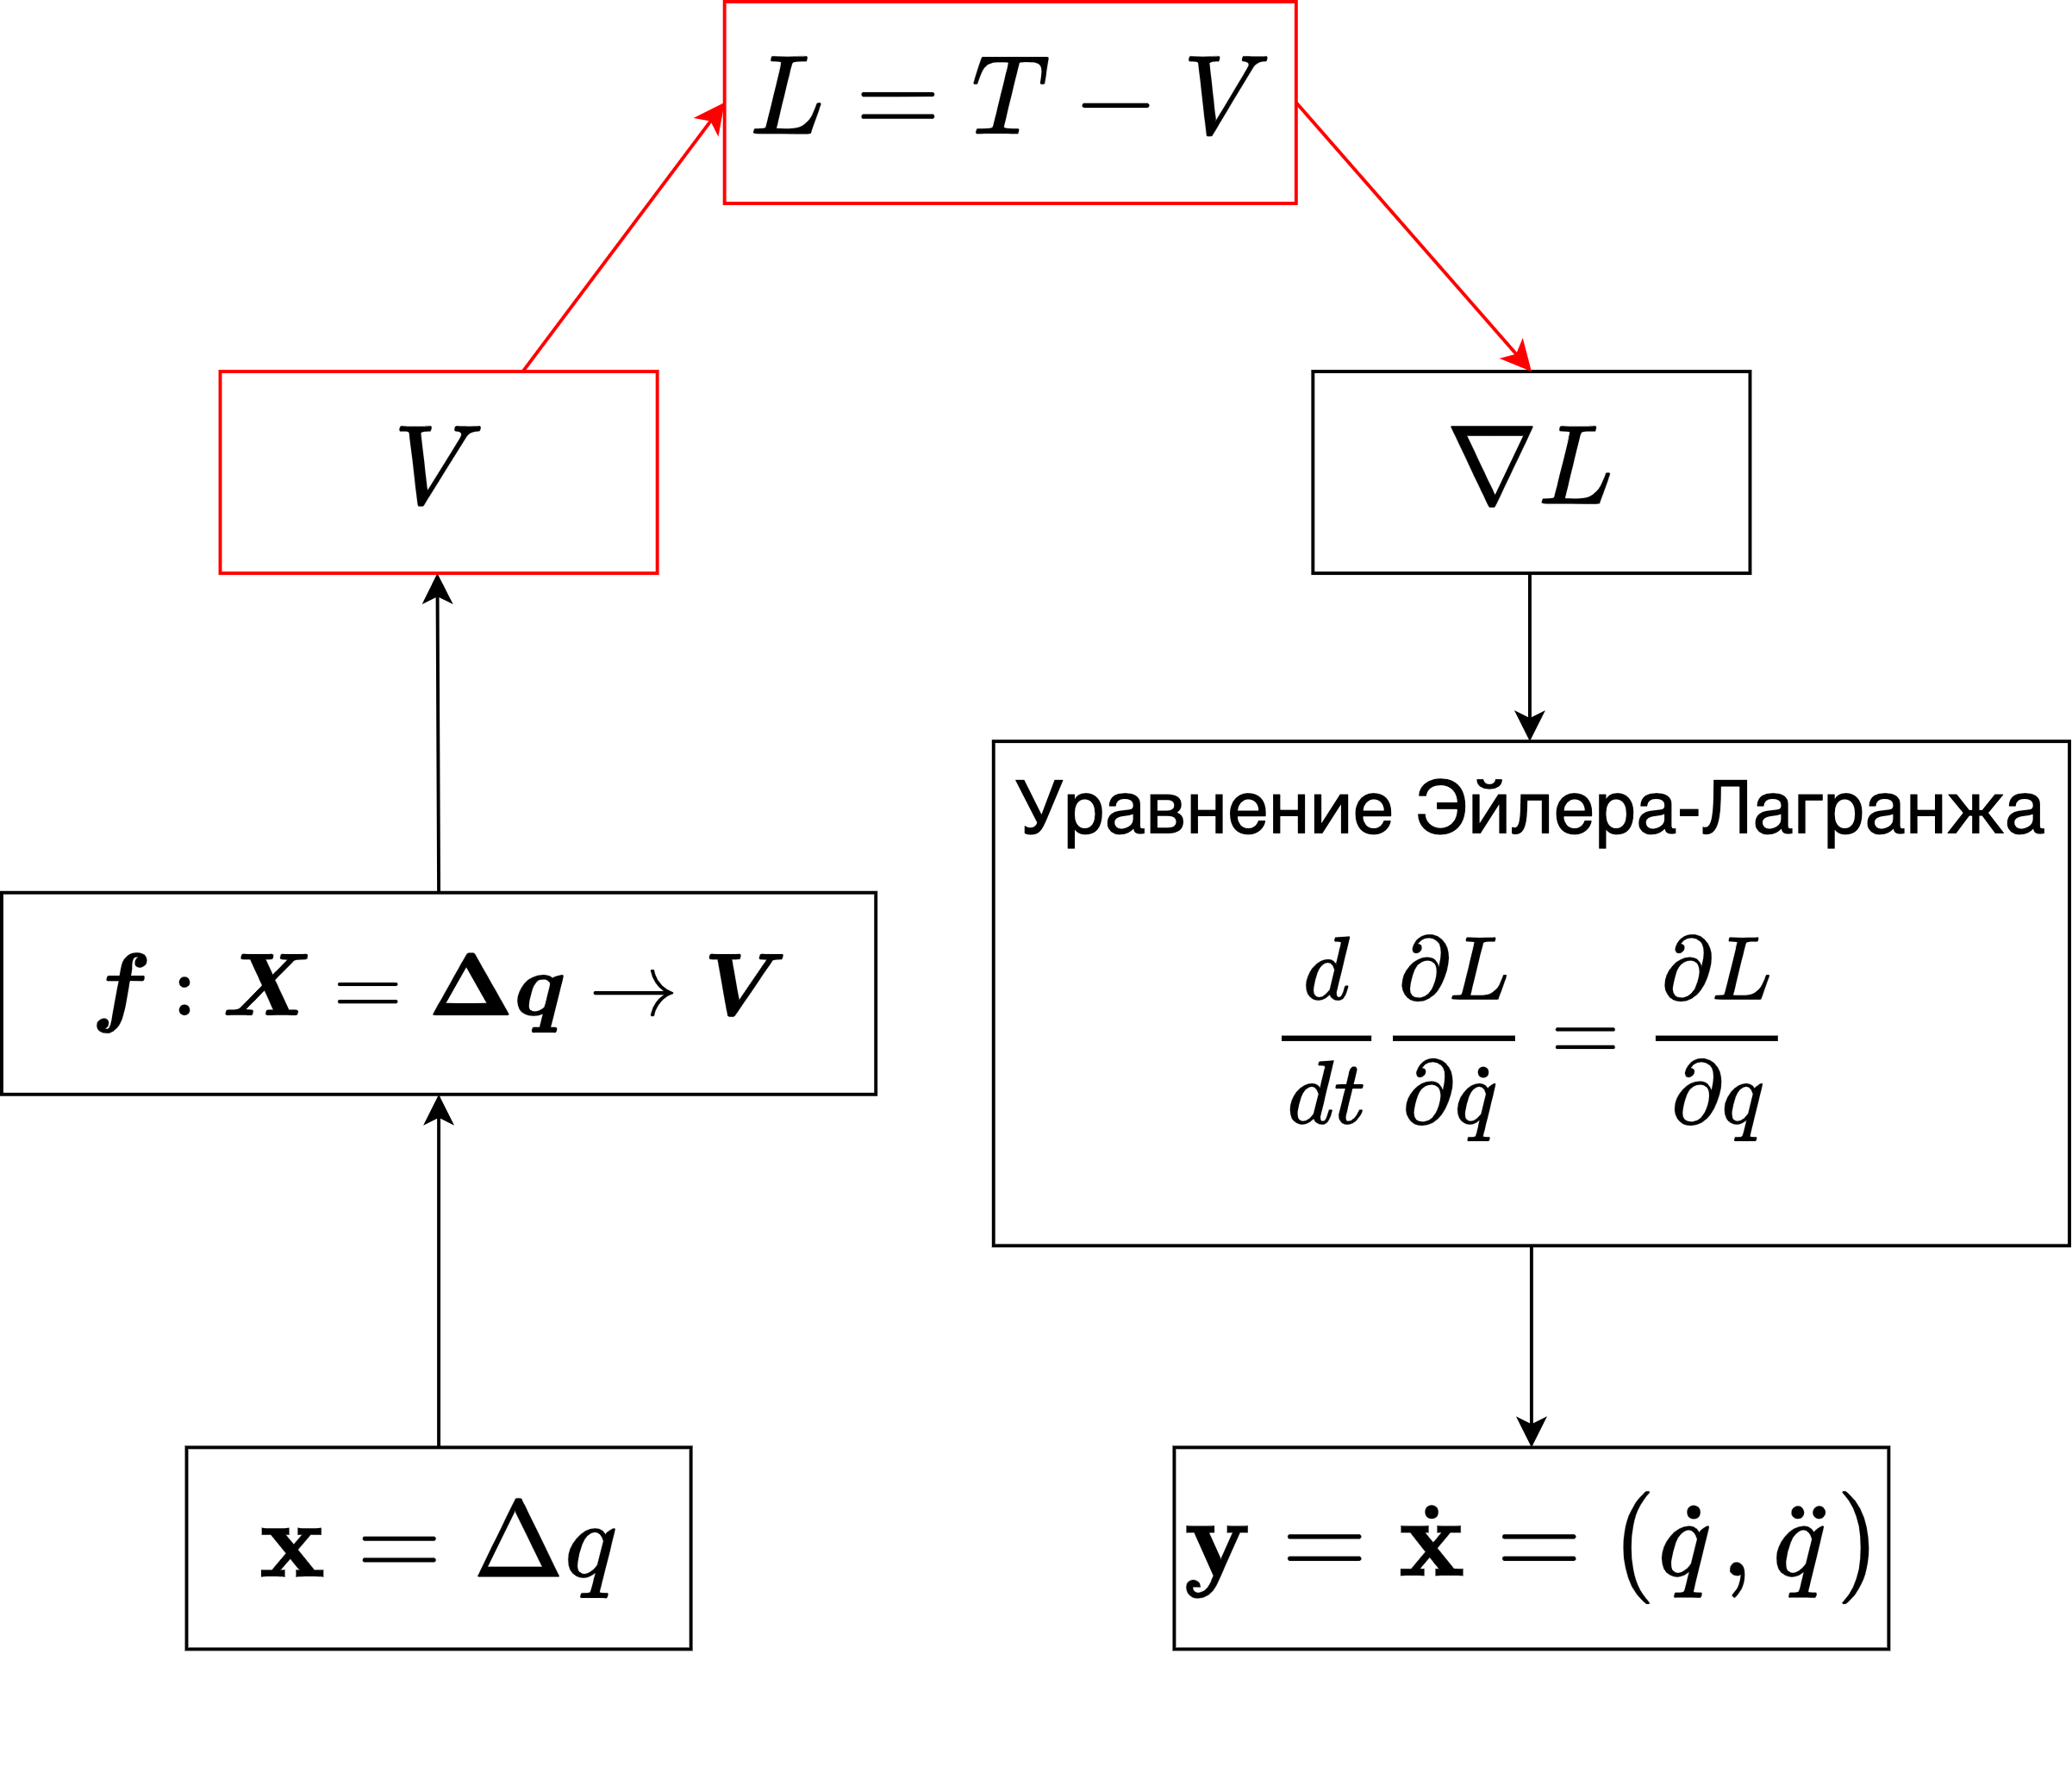
\includegraphics[width=0.95\textwidth]{noether_lnn_scheme.png}
		\caption{Cхема работы Нётеровской LNN}
		%\label{fig:three sin x}
	\end{subfigure}
\caption{Схемы работы LNN (a) и Нётеровской LNN (b) для задачи моделирования динамики физической системы}
\label{fig: lnn_vs_noetherlnn}
\end{figure}

Покажем, что данная модификация LNN сохраняет импульс и момент импульса системы двойного маятника.

\begin{Theorem} (Северилов, 2022)
	Нётеровская LNN учитывает трансляционную симметрию (закон сохранения импульса). Т.е. лагранжиан системы не изменится, если подвергнуть элементы системы перемещению $\bm{\xi}$: 
$$L(\mathbf{\Delta \tilde{q}} , \mathbf{{\dot{\tilde{q}}}} ) = L(\mathbf{\Delta q}, \mathbf{\dot{q}}), ~~\mathbf{\tilde{q}} = \mathbf{q} + \bm{\xi}$$

\end{Theorem}
\begin{Proof}
	Допустим грузы маятника подверглись перемещению $\bm{\xi}$, т.е. обновленные координаты сисетемы примут вид:
	$$\mathbf{\tilde{q}} = \mathbf{q} + \bm{\xi} = \begin{bmatrix}\vec{q}_1 + \vec{\xi} \\\dots\\\vec{q}_r + \vec{\xi}\end{bmatrix},$$ где $r$ -- число координат системы. 
	
	Тогда, учитывая, что $\mathbf{{\dot{\tilde{q}}}}  = \mathbf{\dot{q}}$, лагранжиан обновленной системы:
	$$L(\mathbf{\Delta \tilde{q}}, \mathbf{\dot{\tilde{q}}}) = L(\mathbf{\Delta \tilde{q}}, \mathbf{\dot{q}})  = T(\mathbf{\Delta \tilde{q}}, \mathbf{\dot{q}}) - V(\mathbf{\Delta \tilde{q}})$$
	
	Таким образом, чтобы показать инвариантность лагранжиана относительно перемещения, необходимо показать, что
	$$T(\mathbf{\Delta \tilde{q}}, \mathbf{\dot{q}}) = T(\mathbf{\Delta q}, \mathbf{\dot{q}}),~~ V(\mathbf{\Delta \tilde{q}}) = V(\mathbf{\Delta q})$$
	
	Равенства будут выполнены, если $\mathbf{\Delta \tilde{q}} = \mathbf{\Delta q}$:
	$$\begin{aligned} 
	\Delta \tilde{q}_{i j} &=\sqrt{\left.\left[\left(\vec{q}_{i}+\vec{\xi}\right)-\left(\vec{q}_{j}+\vec{\xi}\right)\right] \cdot\left[\left(\vec{q}_{i}+\vec{\xi}\right)-\left(\vec{q}_{j}+\vec{\xi}\right)\right]\right)} \\ &=\sqrt{\left(\vec{q}_{i}-\vec{q}_{j}\right) \cdot\left(\vec{q}_{i}-\vec{q}_{j}\right)} \\ &= \Delta q_{i j} 
	\end{aligned}$$
	
	Получили, что $L(\mathbf{\Delta \tilde{q}}, \mathbf{\dot{\tilde{q}}}) = L(\mathbf{\Delta q}, \mathbf{\dot{q}})$, т.е. полученный лагранжиан инвариантен относительно перемещения координат -- имеет трансляционную симметрию. Тогда по теореме Нётер из трансляционной симметрии следует закон сохранения импульса.
	
\end{Proof}


\begin{Theorem} (Северилов, 2022)
	Нётеровская LNN учитывает вращательную симметрию (закон сохранения момента импульса). Т.е. лагранжиан системы не изменится, если подвергнуть элементы системы повороту $\mathbf{Q}$: 
	$$L(\mathbf{\Delta \tilde{q}} , \mathbf{{\dot{\tilde{q}}}} ) = L(\mathbf{\Delta q}, \mathbf{\dot{q}}),~~ \mathbf{ \tilde{q}} = \mathbf{Q}\mathbf{ q}$$
\end{Theorem}
\begin{Proof}
	Допустим, элементы системы подверглись повороту матрицей поворота $\mathbf{Q}$, т.е. обновленные координаты сисетемы примут вид $\mathbf{\tilde{q}} = \mathbf{Q}\mathbf{q}$.
	Аналогично теореме 1, достаточно показать, что $$T(\mathbf{\Delta \tilde{q}}, \mathbf{\dot{q}}) = T(\mathbf{\Delta q}, \mathbf{\dot{q}}),~~ V(\mathbf{\Delta \tilde{q}}) = V(\mathbf{\Delta q}),$$
	т.е., что $\mathbf{\Delta \tilde{q}} = \mathbf{\Delta q}$.
	
	Т.к. $\mathbf{Q}$ является матрицей поворота, то $\mathbf{Q}$ -- ортогональная, т.е. $\mathbf{Q}\mathbf{Q}^\mathsf{T} = \mathbf{Q}^\mathsf{T}\mathbf{Q} = \mathbf{I}$. Тогда:
	
	$$\begin{aligned} 
	\Delta\tilde{q}_{i j}
	&=\sqrt{\left(\mathbf{Q} \vec{q_{i}}-\mathbf{Q} \vec{q_{j}}\right) \cdot\left(\mathbf{Q} \vec{q_{i}}-\mathbf{Q} \vec{q_{j}}\right)} \\&=\sqrt{\mathbf{Q}\left(\vec{q_{i}}-\vec{q_{j}}\right) \cdot \mathbf{Q}\left(\vec{q_{i}}-\vec{q_{j}}\right)} 
	\\&=\sqrt{\mathbf{Q} \mathbf{Q}^{T}\left(\vec{q_{i}}-\vec{q_{j}}\right) \cdot\left(\vec{q_{i}}-\vec{q_{j}}\right)} 
	\\&=\sqrt{\left(\vec{q}_{i}-\vec{q}_{j}\right) \cdot\left(\vec{q}_{i}-\vec{q}_{j}\right)} 
	\\&=\Delta q_{i j}
	\end{aligned}$$
	
	Получили, что $L(\mathbf{\Delta \tilde{q}}, \mathbf{\dot{\tilde{q}}}) = L(\mathbf{\Delta q}, \mathbf{\dot{q}})$, т.е. полученный лагранжиан инвариантен относительно поворота координат -- имеет вращательную симметрию. Тогда по теореме Нётер из вращательной симметрии следует закон сохранения момента импульса.
\end{Proof}

В качестве нейронной сети $f: \mathbf{X} = (\mathbf{\Delta q}) \rightarrow \mathbf{V}$ аналогично LNN берется полносвязная сеть с 3-мя слоями. Таким образом, для заданных координат  $(\mathbf{q}, \mathbf{\dot{q}})$ имеем модель с априорными знанями о законе сохранения энергии, импульса и момента импульса, которой можем получить динамику параметров $(\mathbf{\dot{q}}, \mathbf{\ddot{q}})$. 

\section{Система двойного маятника}

В качестве моделируемой физической системы взята система двойного маятника (Рис. \ref{fig:pendulum_system}). Двойной маятник образуется путем присоединения одного маятника к другому. Каждый маятник состоит из груза, соединенного с безмассовым жестким стержнем, который может двигаться только в вертикальной плоскости. Ось первого маятника закреплена в точке $O$. Все движения без трения.

В данном случае координатами $\textbf{q}$ являются углы между стержнями маятника и вертикальной осью $$\textbf{q} = (\mathbf{\theta}_1, \mathbf{\theta}_2)$$


\begin{figure}[H]
	\centering
	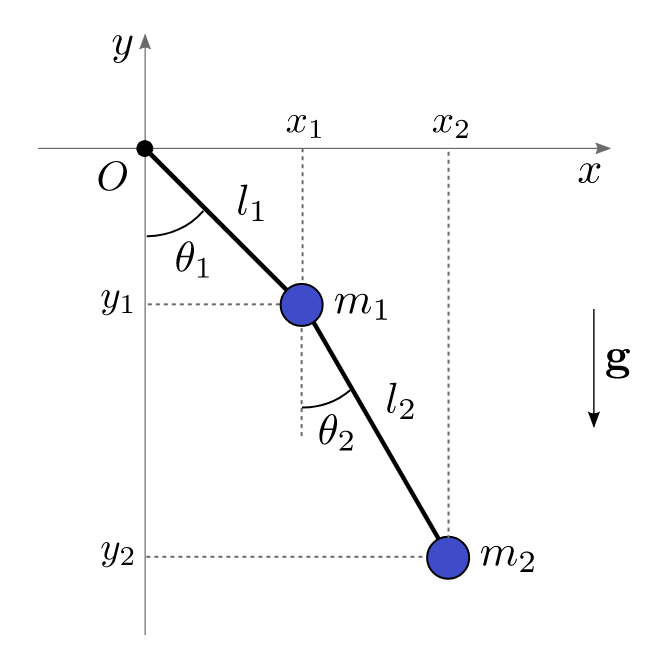
\includegraphics[width=0.6\textwidth]{double_pendulum_scheme.png}
	\caption{Cхема физической системы двойного маятника}
	\label{fig:pendulum_system}
\end{figure}

\subsection{Лагранжиан системы}

Примем точку $O$ за начало декартовой системы координат с осью $x$, направленной вдоль горизонтального направления, и осью $y$, направленной вертикально вверх. Пусть $\theta_1$ и $\theta_2$ -- углы, которые первый и второй стержни образуют с вертикальным направлением соответственно. Как видно на рисунке \ref{fig:pendulum_system}, положения грузов задаются следующим образом:

$$
\begin{aligned}
x_{1} & =l_{1} \sin \theta_{1}, && y_{1}=-l_{1} \cos \theta_{1}, \\
x_{2} & =l_{1} \sin \theta_{1}+l_{2} \sin \theta_{2}, &&  y_{2}=-l_{1} \cos \theta_{1}-l_{2} \cos \theta_{2}
\end{aligned}
$$

Дифференцируя приведенные выше величины по времени, получаем скорости грузов:

$$
\begin{aligned}
\dot{x}_{1} &=l_{1} \dot{\theta}_{1} \cos \theta_{1} & & \dot{y}_{1}=l_{1} \dot{\theta}_{1} \sin \theta_{1} \\
\dot{x}_{2} &=l_{1} \dot{\theta}_{1} \cos \theta_{1}+l_{2} \dot{\theta}_{2} \cos \theta_{2} & & \dot{y}_{2}=l_{1} \dot{\theta}_{1} \sin \theta_{1}+l_{2} \dot{\theta}_{2} \sin \theta_{2}
\end{aligned}
$$

Данная система имеет лагранжиан:
$$
\begin{aligned}
L=\frac{1}{2}\left(m_{1}+m_{2}\right) l_{1}^{2} \dot{\theta}_{1}^{2} &+\frac{1}{2} m_{2} l_{2}^{2} \dot{\theta}_{2}^{2}+m_{2} l_{1} l_{2} \dot{\theta}_{1} \dot{\theta}_{2} \cos \left(\theta_{1}-\theta_{2}\right) \\
&+\left(m_{1}+m_{2}\right) g l_{1} \cos \theta_{1}+m_{2} g l_{2} \cos \theta_{2}
\end{aligned}
$$

Лагранжиан для двойного маятника определяется выражением $L=T - V$, где $T$ и $V$ -- кинетическая и потенциальная энергии системы соответственно. Кинетическая энергия $T$ определяется выражением:
$$
\begin{aligned}
T &=\frac{1}{2} m_{1} v_{1}^{2}+\frac{1}{2} m_{2} v_{2}^{2} \\
&=\frac{1}{2} m_{1}\left(\dot{x}_{1}^{2}+\dot{y}_{1}^{2}\right)+\frac{1}{2} m_{2}\left(\dot{x}_{2}^{2}+\dot{y}_{2}^{2}\right) \\
&=\frac{1}{2} m_{1} l_{1}^{2} \dot{\theta}_{1}^{2}+\frac{1}{2} m_{2}\left[l_{1}^{2} \dot{\theta}_{1}^{2}+l_{2}^{2} \dot{\theta}_{2}^{2}+2 l_{1} l_{2} \dot{\theta}_{1} \dot{\theta}_{2} \cos \left(\theta_{1}-\theta_{2}\right)\right]
\end{aligned}
$$

В выражении выше использован факт, что $\cos \theta_{1} \cos \theta_{2}+\sin \theta_{1} \sin \theta_{2}=\cos \left(\theta_{1}-\theta_{2}\right)$. Потенциальная энергия $V$ определяется выражением:
$$
\begin{aligned}
V &=m_{1} g y_{1}+m_{2} g y_{2} \\
&=-m_{1} g l_{1} \cos \theta_{1}-m_{2} g\left(l_{1} \cos \theta_{1}+l_{2} \cos \theta_{2}\right) \\
&=-\left(m_{1}+m_{2}\right) g l_{1} \cos \theta_{1}-m_{2} g l_{2} \cos \theta_{2}
\end{aligned}
$$
Таким образом, Лагранжиан системы:
$$
\begin{aligned}
L=\frac{1}{2}\left(m_{1}+m_{2}\right) l_{1}^{2} \dot{\theta}_{1}^{2} &+\frac{1}{2} m_{2} l_{2}^{2} \dot{\theta}_{2}^{2}+m_{2} l_{1} l_{2} \dot{\theta}_{1} \dot{\theta}_{2} \cos \left(\theta_{1}-\theta_{2}\right) \\
&+\left(m_{1}+m_{2}\right) g l_{1} \cos \theta_{1}+m_{2} g l_{2} \cos \theta_{2}
\end{aligned}
$$


\subsection{Аналитическое решение получения динамики системы}
После подставления полученного лагранжиана в уравнение Эйлера-Лагранжа выражение сводится к системе дифференциальных уравнений \cite{double_pendulum}

$$
\begin{array}{c}
\frac{d}{d t}\left(\begin{array}{c}
\theta_{1} \\
\theta_{2} \\
\dot{\theta}_{1} \\
\dot{\theta}_{2}
\end{array}\right)=\left(\begin{array}{c}
\omega_{1} \\
\omega_{2} \\
g_{1}\left(\theta_{1}, \theta_{2}, \dot{\theta}_{1}, \dot{\theta}_{2}\right) \\
g_{2}\left(\theta_{1}, \theta_{2}, \dot{\theta}_{1}, \dot{\theta}_{2}\right)
\end{array}\right)
\end{array}
$$
где $g_{1}=\frac{f_{1}-\alpha_{1} f_{2}}{1-\alpha_{1} \alpha_{2}} \quad, g_{2}=\frac{-\alpha_{2} f_{1}+f_{2}}{1-\alpha_{1} \alpha_{2}}$, $\alpha_{i}=\alpha_{i}\left(\theta_{1}, \theta_{2}\right)$ и $f_{i}=f_{i}\left(\theta_{1}, \theta_{2}, \dot{\theta}_{1}, \dot{\theta}_{2}\right)$ для $i=1,2$

$$
\begin{aligned}{l}
\alpha_{1}\left(\theta_{1}, \theta_{2}\right) & =\frac{l_{2}}{l_{1}}\left(\frac{m_{2}}{m_{1}+m_{2}}\right) \\
\alpha_{2}\left(\theta_{1}, \theta_{2}\right) &=\frac{l_{1}}{l_{2}} \cos \left(\theta_{1}-\theta_{2}\right) \\
f_{1}\left(\theta_{1}, \theta_{2}, \dot{\theta}_{1}, \dot{\theta}_{2}\right) & =-\frac{l_{2}}{l_{1}}\left(\frac{m_{2}}{m_{1}+m_{2}}\right) \dot{\theta}_{2}^{2} \sin \left(\theta_{1}-\theta_{2}\right)-\frac{g}{l_{1}} \sin \theta_{1} \\
f_{2}\left(\theta_{1}, \theta_{2}, \dot{\theta}_{1}, \dot{\theta}_{2}\right) & =\frac{l_{1}}{l_{2}} \dot{\theta}_{1}^{2} \sin \left(\theta_{1}-\theta_{2}\right)-\frac{g}{l_{2}} \sin \theta_{2}
\end{aligned}
$$
Полученная система дифференциальных уравнений может быть решена численно с помощью метода Рунге-Кутты 4 порядка.

\subsection{Данные}

Для обучения моделей были сгенерированы 20 траекторий движениями двойного маятника из разных начальных состояний $\mathbf{x}_0$ длиной 1500 моментов времени по 0.01 секунде. Длины стержней и массы грузов приняты равными 1. Генерация данных производилась на основе решения системы дифференциальных уравнений, описывающих динамику системы, с помощью метода рунге-Кутты 4 порядка.

На рисунке \ref{fig:coords_vis} представлена визуализация сгнерированных координат $\theta_1, \theta_2$ для одной из траекторий. Цвет означает угол наклона нижнего стержня маятника: зеленый, если угол $\theta_2 > 0$, синий, если $\theta_2 < 0$.
 
\begin{figure}[H]
	\centering
	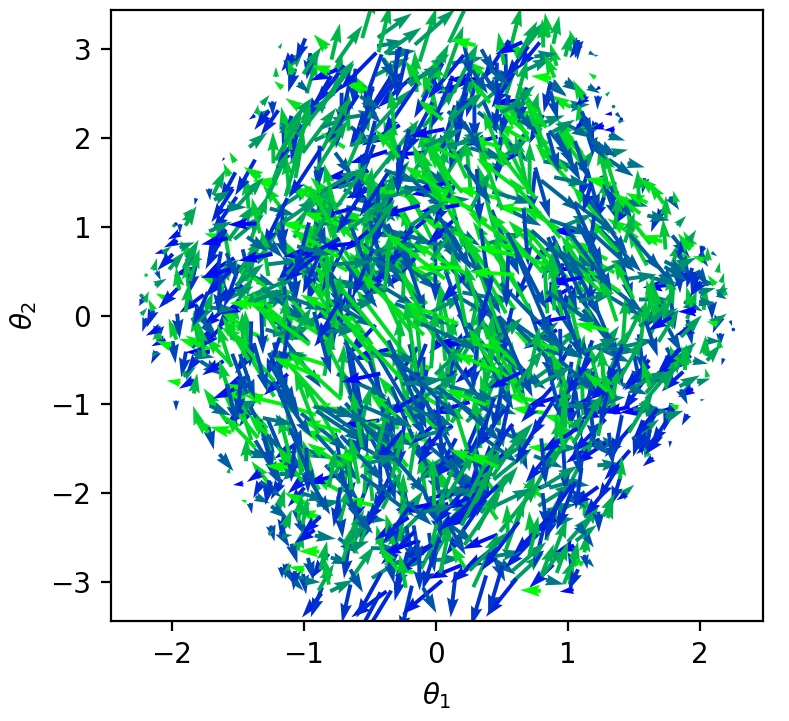
\includegraphics[width=0.6\textwidth]{train_test_data_vis.png}
	\caption{Визуализация данных координат $\theta_1, \theta_2$ системы двойного маятника}
	\label{fig:coords_vis}
\end{figure}


\section{Вычислительный эксперимент}
В рамках вычислительного эксперимента написан программный комплекс для решения поставленных задач~\cite{source_code}.

\subsection{Исследуемые модели нейронных сетей}
В качестве исследуемых моделей для сравнения моделирования динамики системы были использованы полносвязная нейронная сеть (FC), сеть с долговременной кратковременной памятью (LSTM), Лагранжева нейронная сеть и Нётеровская LNN, учитывающая трансляционную и вращательную симметрии. В качестве истинной динамики системы взята динамика, полученная аналитическим решением методом Рунге-Кутты 4 порядка.

В таблице \ref{tab:models} представлены сравниваемые модели. FC является простейшей нейронной сетью с малым количеством параметров. LSTM имеет значительно большее количество параметров, чем полносвязный сеть, но больше подходит для работы с последовательностями (в нашем случае траекториями) \cite{lstm}. LNN является полносвязной сетью, но имеет априорное знание о законе сохранения энергии. Нётеровская LNN тоже является полносвязной сетью, но имеющей априорное знание о трех законах сохранения: энергии, имупльса, момента импульса.

\begin{table}[h]
	\centering
	\begin{tabular}{c|c}
		\textbf{Аналитическое решение}                                                                              & Метод Рунге-Кутты 4 порядка \\ \hline
		\textbf{\begin{tabular}[c]{@{}c@{}}Полносвязная нейронная \\ сеть (FC)\end{tabular}}                        &            \begin{tabular}[c]{@{}c@{}}$f: \boldsymbol{X} = (\boldsymbol{q}, \boldsymbol{\dot{q}}) \rightarrow \boldsymbol{Y}$, \\$f = \sigma(... \boldsymbol{W}^T \sigma(\boldsymbol{W}^T\boldsymbol{x} + \boldsymbol{b}))$ \end{tabular}                          \\ \hline
		\textbf{\begin{tabular}[c]{@{}c@{}}Нейронная сеть с долгой \\ краткосрочной памятью \\ (LSTM)\end{tabular}} &        \begin{tabular}[c]{@{}c@{}}$h: \boldsymbol{X} = (\boldsymbol{q}, \boldsymbol{\dot{q}}) \rightarrow \boldsymbol{Y}$, \\
			$\begin{aligned} f_{t} &=\sigma_{g}\left(W_{f} x_{t}+U_{f} h_{t-1}+b_{f}\right) \\ i_{t} &=\sigma_{g}\left(W_{i} x_{t}+U_{i} h_{t-1}+b_{i}\right) \\ o_{t} &=\sigma_{g}\left(W_{o} x_{t}+U_{o} h_{t-1}+b_{o}\right) \\ c_{t} &=f_{t} \circ c_{t-1}+i_{t} \circ \sigma_{c}\left(W_{c} x_{t}+U_{c} h_{t-1}+b_{c}\right) \\ h_{t} &=o_{t} \circ \sigma_{h}\left(c_{t}\right) \end{aligned}$  
		\end{tabular}                  \\ \hline
		\textbf{LNN}     &            \begin{tabular}[c]{@{}c@{}}$f: \boldsymbol{X} = (\boldsymbol{q}, \boldsymbol{\dot{q}}) \rightarrow \boldsymbol{L}$, \\$\ddot{q} =\left(\nabla_{\dot{q}} \nabla_{\dot{q}}^{\top} L\right)^{-1}\left[\nabla_{q} L-\left(\nabla_{q} \nabla_{\dot{q}}^{\top} L\right) \dot{q}\right]$ \end{tabular}                \\ \hline
		\textbf{Нётеровская LNN}                                                                                    &       \begin{tabular}[c]{@{}c@{}}$f: \boldsymbol{X} =(\boldsymbol{q}, \boldsymbol{\dot{q}}) \rightarrow \boldsymbol{V}$, \\$L = T - V$, 	\\$\ddot{q} =\left(\nabla_{\dot{q}} \nabla_{\dot{q}}^{\top} L\right)^{-1}\left[\nabla_{q} L-\left(\nabla_{q} \nabla_{\dot{q}}^{\top} L\right) \dot{q}\right]$ \end{tabular}                         
	\end{tabular}
	\label{tab:models}
	\caption{Сравниваемые методы моделирования динамики системы двойного маятника}
\end{table}

\subsection{Результаты}
Результаты моделирования динамики системы двойного маятника различными видами нейронных сетей представлены в таблице \ref{res_table}. Выборка состоит из 10 траекторий, сгенерированных на основе решения методом Рунге-Кутты 4 порядка.

\begin{table}[h]
	\centering
	\begin{tabular}{c|c}
		FC              & $1.57 \pm 0.53$                          \\ \hline
		LSTM            & $2.42  \pm 0.79$                            \\ \hline
		LNN             & $1.32\pm 0.91$                            \\ \hline
		Нётеровская LNN & \textbf{ 1.28} $ \pm 0.66$
	\end{tabular}
	\label{res_table}
	\caption{Средняя ошибка RMSE между предсказанной динамикой системы нейронной сетью и динамикой системы, полученной аналитическим решением.}
\end{table}

Сравнивания результаты LNN и FC, LSTM, можем сделать вывод, что модель, имеющая априорные знания о физике системы имеет выше точность моделирования динамики системы.
Сравнивая результаты LNN и Нётеровской LNN, можем сделать вывод, что добавление дополнительных априорных знаний о физике системы повышает точность моделирования динамики системы


На рис \ref{fig:result_graphs} представлены траектории движения нижнего груза двойного маятника, полученные аналитическим решением и рассматриваемыми нейронными сетями. Динамика, предсказанная моделями LNN и Нётеровской LNN, наиболее близка к динамике, полученной аналитическим решением. Это подтверждает гипотезу, что добавление априорных знаний о лагранжиане системы повышает точность предсказания динамики системы (траектории движения маятника).

\begin{figure}[H]
	\centering
	\begin{subfigure}[b]{0.49\textwidth}
		\centering
		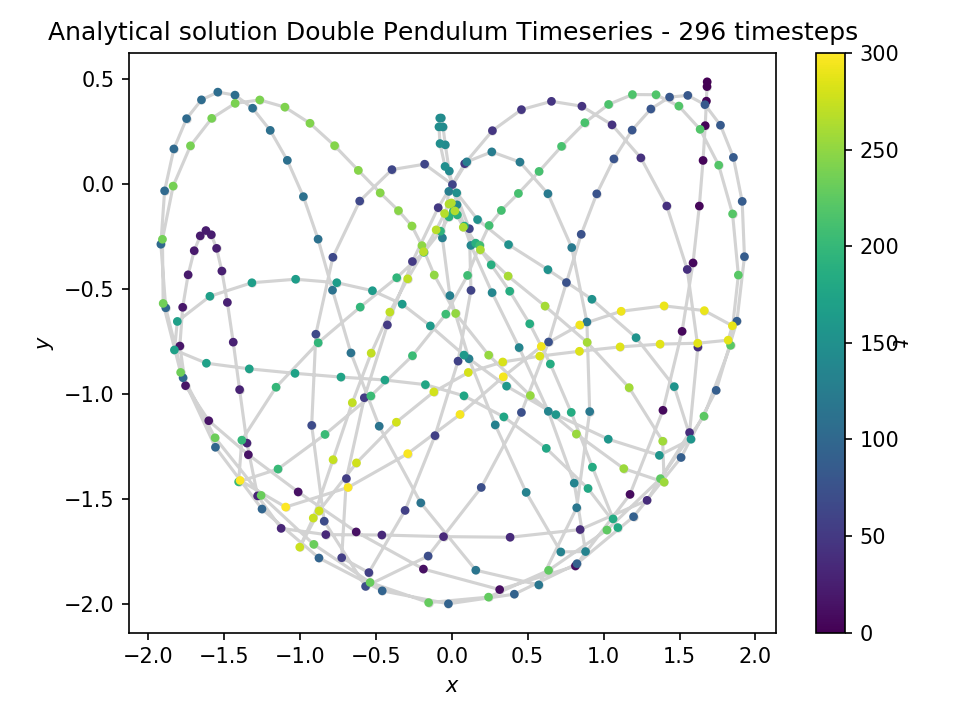
\includegraphics[width=\textwidth]{predicted_trajectory_Analytical solution.png}
		\caption{Аналитическое решение}
		\label{fig:y equals x}
	\end{subfigure}
	\hfill
	\begin{subfigure}[b]{0.49\textwidth}
		\centering
		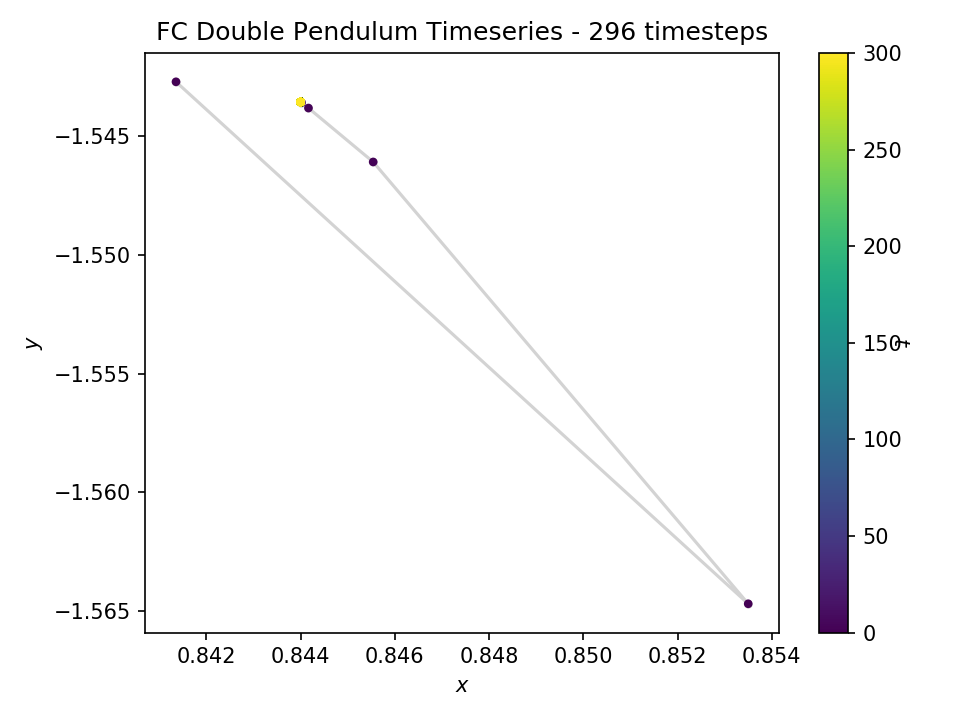
\includegraphics[width=\textwidth]{predicted_trajectory_FC.png}
		\caption{FC}
		\label{fig:three sin x}
	\end{subfigure}
	\hfill
	\vfill
	\begin{subfigure}[b]{0.49\textwidth}
		\centering
		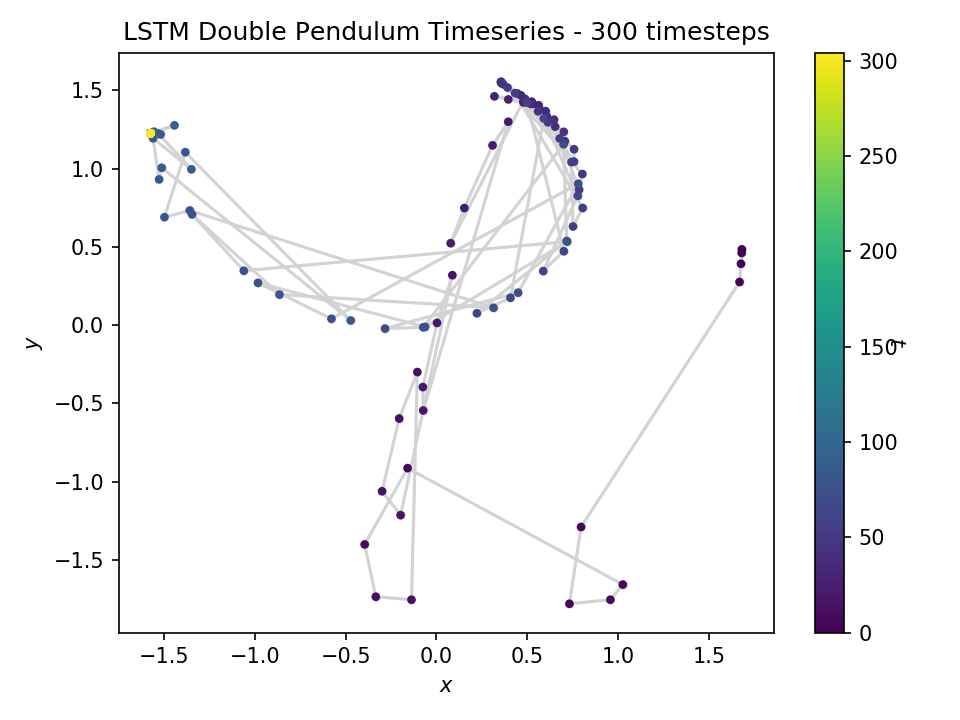
\includegraphics[width=\textwidth]{predicted_trajectory_LSTM.png}
		\caption{LSTM}
		\label{fig:three sin x}
	\end{subfigure}
	\hfill
	\begin{subfigure}[b]{0.49\textwidth}
		\centering
		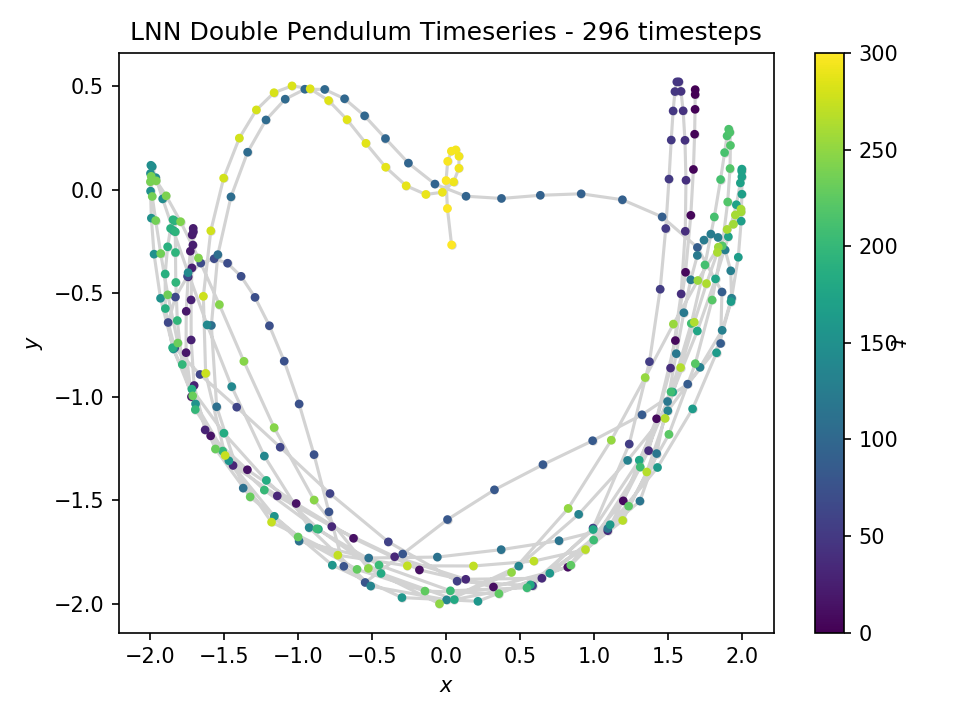
\includegraphics[width=\textwidth]{predicted_trajectory_LNN.png}
		\caption{LNN}
		\label{fig:five over x}
	\end{subfigure}
	\begin{subfigure}[b]{0.49\textwidth}
		\centering
		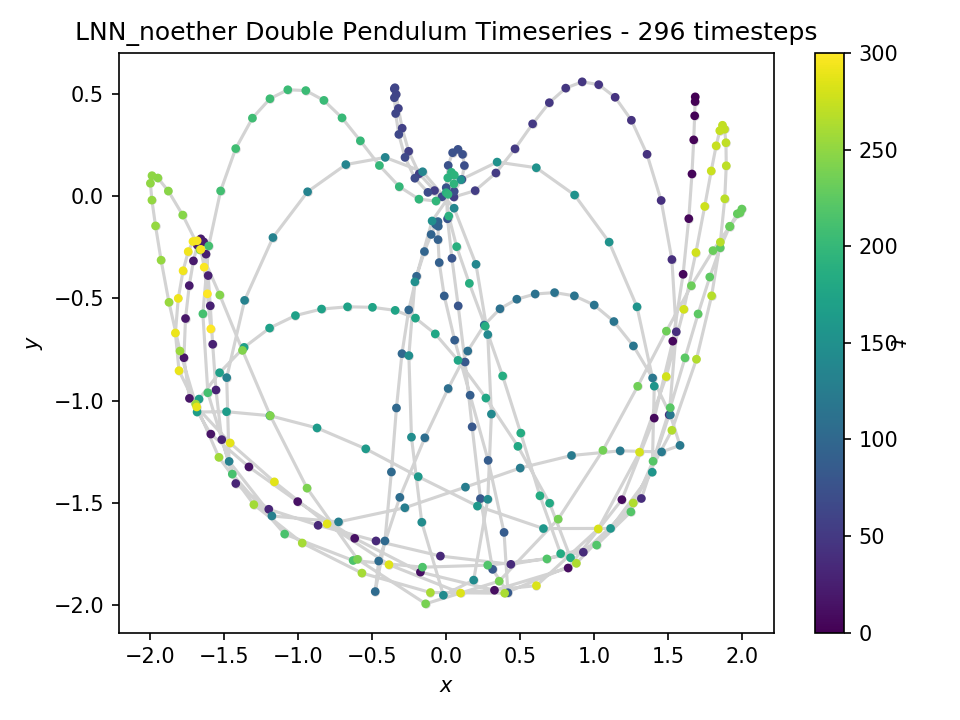
\includegraphics[width=\textwidth]{predicted_trajectory_LNN_noether.png}
		\caption{Нётеровская LNN}
		\label{fig:five over x}
	\end{subfigure}
	\caption{Моделирование динамики системы двойного маятника различными видами нейронных сетей: аналитическое решение, полносвязная нейронная сеть, LSTM, LNN и Нётеровская LNN.}
	\label{fig:result_graphs}
\end{figure}


\section{Заключение}
	В данной работе предложена Нётеровская LNN, которая в дополнение к закону сохранения энергии учитывает закон сохранения импульса и момента импульса. Также были доказаны теоремы, подтверждающие корректность учета закона сохранения импульса и момента импульса. На основе экспериментов по моделированию динамики системы двойного маятника показано, что добавление априорных знаний о физике системы повышает точность моделирования динамики физической системы. 
	
	Данные результаты показывают адекватность использования моделей с априорными знаниями о физике системы и открывает новые пути развития данных моделей. В качестве дальнейших исследований предлагается использование более сложных моделей нейронных сетей в основе LNN: использование реккурентных, сверточных сетей вместо только полносвязных.

\newpage

%\nocite{*}
\newpage

\bibliographystyle{gost71s}
\bibliography{mtaibiblio}
\addcontentsline{toc}{section}{Список литературы}

\end{document}
